\documentclass[a4paper, 12pt]{article}

\usepackage{babel}
\usepackage{enumitem}
\usepackage{times}
\usepackage{graphicx}
\usepackage{geometry}
	\geometry{left = 3cm, top = 3cm, right = 3cm, bottom = 3cm}
\usepackage{float}
\usepackage{setspace}
	\setstretch{1.5}
\usepackage{listings}

\title{CHAPTER 4}
\author{John Kevin Giraldi (1184049)}
\date{14 Desember 2019}

\begin{document}

\maketitle

\section{TEORI}
\subsection{ Sejarah dan Contoh Pengelolaan File CSV}
\paragraph{CSV atau Comma Separated Value adalah salah satu tipe file yang digunakan dalam pengolahan informasi yang menghasilkan spreadsheet untuk diproses lebih lanjut melalui mesin analitik. CSV pun dianggap sebagai file yang agnostik karena dapat digunakan oleh berbagai database untuk proses backup data. Format data pada CSV memudahkan penggunaanya dalam melakukan penginputan data ke database. CSV dapat digunakan dalam standar file ASCII, jadi setiap record dipisahkan dengan tanda(,) atau titik koma(;).File CSV digunakan untuk menyimpan informasi yang dipisahkan oleh koma, bukan menyimpan informasi dalam kolom.Dan jika teks dan angka disimpan dalam file csv maka mudah untuk memindahkannya dari satu program ke program lain.}
Contoh: \\

\subsection{Aplikasi Pembuat File CSV}
Ada beberapa aplikasi yang menghasilkan file CSV antara lain:
\begin{itemize}
    \item Ms.Excel
    \item Google sheet
    \item Notepad
\end{itemize}

\subsection{Cara Menulis dan Membaca File CSV di Excel atau Spreadsheet}
\begin{enumerate}
    \item Buka Program Excel atau Spreadsheet Sejenis.
    \item Masukkan Data Pada Baris dan Kolom
    \item Save as, dan save file dengan format .csv
\end{enumerate}

\subsection{Sejarah Library CSV}
\paragraph{Format data yang disebut CSV (Comma Separated Values) adalah format data impor dan ekspor yang paling umum untuk spreadsheet dan basis data. Format CSV digunakan untuk menggambarkan format dengan cara yang standar di RFC 4180 . Kurangnya standar yang didefinisikan dengan baik berarti bahwa perbedaan harus terdapat dalam data yang diproduksi dan dipakai oleh aplikasi yang berbeda.}

\subsection{Sejarah library Pandas}
\paragraph{Merupakan library analisis data yang mempunyai struktur data , library pandas diperlukan untuk mengubah bentuk data bahasa pemrograman menjadi bentuk tabel.}
\subsection{Fungsi-fungsi yang terdapat pada library CSV}
\begin{enumerate}
\item Reader
\paragraph{} Fungsi ini digunakan untuk membaca isi file berformat CSV dari list.
\newpage\begin{figure}[ht]
\centerline{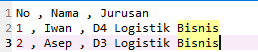
\includegraphics[width=10cm]{figure/1.PNG}}
\end{figure}
\item DictReader
\paragraph{}  Fungsi ini digunakan untuk membaca isi file berformat CSV dari dictionary.
\begin{figure}[ht]
\centerline{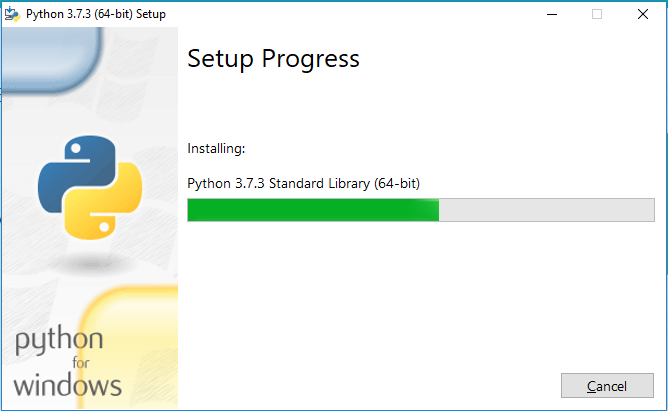
\includegraphics[width=10cm]{figure/2.PNG}}
\end{figure}
\item Write
\paragraph{} Fungsi ini digunakan untuk menulis file berformat CSV dari list.
\begin{figure}[ht]
\centerline{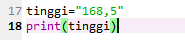
\includegraphics[width=15cm]{figure/3.PNG}}
\end{figure}
\newpage\item DictWrite
\paragraph{}  Fungsi ini digunakan untuk menulis file berformat CSV dari dictionary.
\begin{figure}[ht]
\centerline{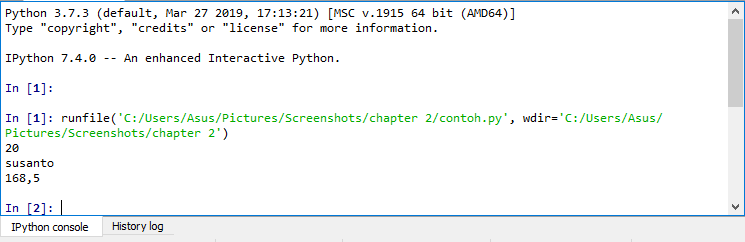
\includegraphics[width=15cm]{figure/4.PNG}}
\end{figure}
\end{enumerate}

\subsection{Fungsi-fungsi yang terdpat pada library Pandas}
\begin{enumerate}
\item Read\_csv
\paragraph{} Fungsi ini digunakan untuk membaca isi file berformat CSV.
\begin{figure}[ht]
\centerline{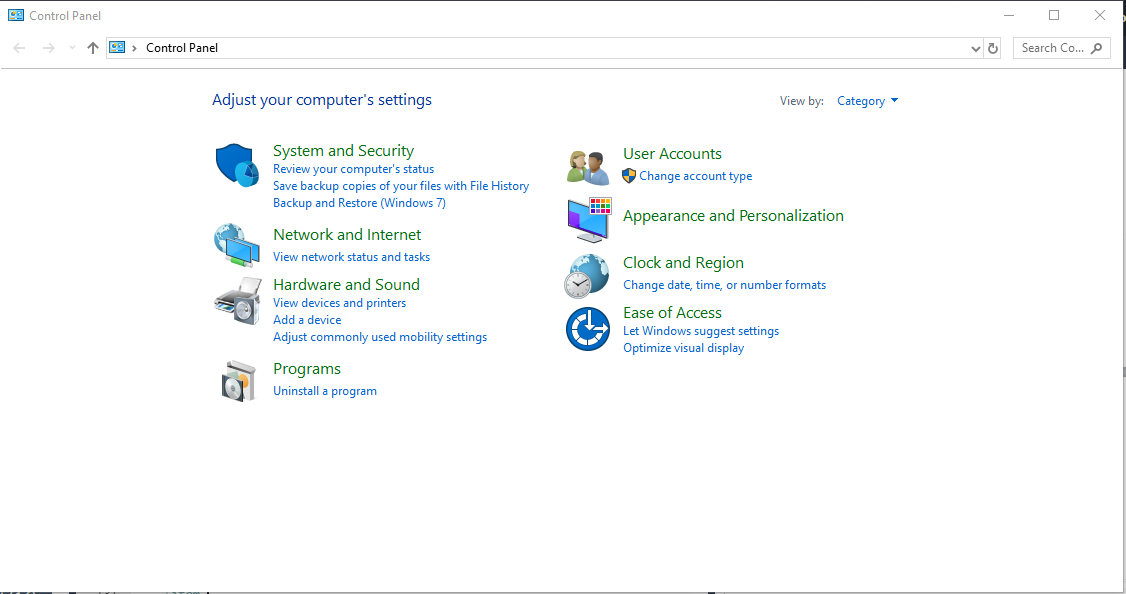
\includegraphics[width=10cm]{figure/5.PNG}}
\end{figure}
\item To\_csv
\paragraph{} Fungsi ini digunakan untuk menulis file berformat CSV.
\begin{figure}[ht]
\centerline{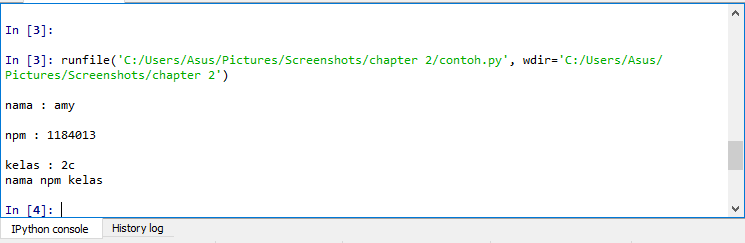
\includegraphics[width=10cm]{figure/6.PNG}}
\end{figure}
\end{enumerate}
\end{document}